\documentclass{article}

% Load amsmath first so the style's author separator \And takes precedence.
\usepackage{amsmath,amssymb}
\usepackage[preprint]{neurips_2025}
\usepackage[utf8]{inputenc}
\usepackage[T1]{fontenc}
\usepackage{booktabs,tabularx,array}
\usepackage{microtype}
\usepackage{graphicx}
\usepackage{capt-of}
\usepackage{flafter}
\usepackage{enumitem}
\usepackage{hyperref}

\newcolumntype{Y}{>{\raggedright\arraybackslash}X}
\newcolumntype{P}[1]{>{\raggedright\arraybackslash}p{#1}}
\setlist[enumerate]{leftmargin=1.8em,itemsep=2pt,topsep=2pt}

% Keep the artwork and caption together, directly above the discussion.
\newenvironment{inlinefigure}{%
  \par\addvspace{\intextsep}%
  \noindent\begin{minipage}[b]{\linewidth}%
  \centering
}{%
  \end{minipage}\par\nopagebreak[4]%
}

\hypersetup{
  colorlinks=true,
  linkcolor=blue,
  citecolor=blue,
  urlcolor=blue,
  pdftitle={PeerSieve: Sketch-Filtered Compressed Streaming for Byzantine-Resilient Decentralized LLM Tuning},
  pdfauthor={Natthanan Bhukan and Germain Dal}
}

\title{PeerSieve: Sketch-Filtered Compressed Streaming\\for Byzantine-Resilient Decentralized LLM Tuning}

\author{%
  Natthanan Bhukan \\
  Tsinghua University \\
  2025280434 \\
  \href{mailto:panyx25@mails.tsinghua.edu.cn}{\texttt{panyx25@mails.tsinghua.edu.cn}} \\
  \And
  Germain Dal \\
  Tsinghua University \\
  2025280175 \\
  \href{mailto:xhm25@mails.tsinghua.edu.cn}{\texttt{xhm25@mails.tsinghua.edu.cn}} \\
}

\begin{document}
\raggedbottom
\maketitle

\section{Introduction}
\label{sec:motivation}

In decentralized federated learning (DFL), each peer trains on local data, exchanges models or updates with its neighbors, and aggregates what it receives without a central server. Byzantine peers may send arbitrary updates, but even honest updates can disagree when peers train on different data. A receiver must decide which updates to use without treating every disagreement as evidence of an attack.

Existing defenses differ in what they use as a reference. TrustGraph-DFL~\cite{trustgraph2026} scores received updates by cosine similarity to the receiver's held-out validation gradient. It gives zero weight to updates with nonpositive scores and uses the normalized positive scores to blend a weighted average of its neighbors' models with its own. FLTrust~\cite{cao2021fltrust} also weights received updates by positive cosine similarity, but its reference is an update computed by a central server on a small trusted dataset. The server rescales contributing updates to the reference norm before averaging them. BALANCE~\cite{fang2024balance} needs neither a server nor a validation set, since each receiver averages only the neighbor models within a round-dependent distance threshold of its own locally trained model, then blends that average with its own model.

Each of these defenses receives the full model or update before deciding whether to use it. For TinyLlama-1.1B with low-rank adaptation (LoRA) at rank 128, one update takes 385~MiB in FP32. In our batched TrustGraph-DFL baseline, a peer receives six updates per round, or 2,310~MiB (Table~\ref{tab:round}). At $1$~Gb/s, we estimate 19.4~s for the transfer alone. The example shows four problems:
\begin{enumerate}
  \item \textbf{Rejected updates still cost bandwidth.} If the receiver rejects two updates, it has already received 770~MiB it will not use.
  \item \textbf{Useful updates are still large.} Top-$k$ compression~\cite{karimireddy2019efsgd} sends only the largest changes by absolute value. Dropping the smaller changes can make the receiver reject an update it would have accepted in full.
  \item \textbf{More neighbors mean more buffers.} The batched baseline keeps one full update per neighbor in GPU memory. Checking updates one at a time saves memory, but the receiver must check the whole update before adding any of it to the running sum.
  \item \textbf{The same neighbor can send again.} Rejecting an update does not stop the receiver from downloading the next one. Banning a neighbor after one low score could exclude an honest peer.
\end{enumerate}

\begin{inlinefigure}
  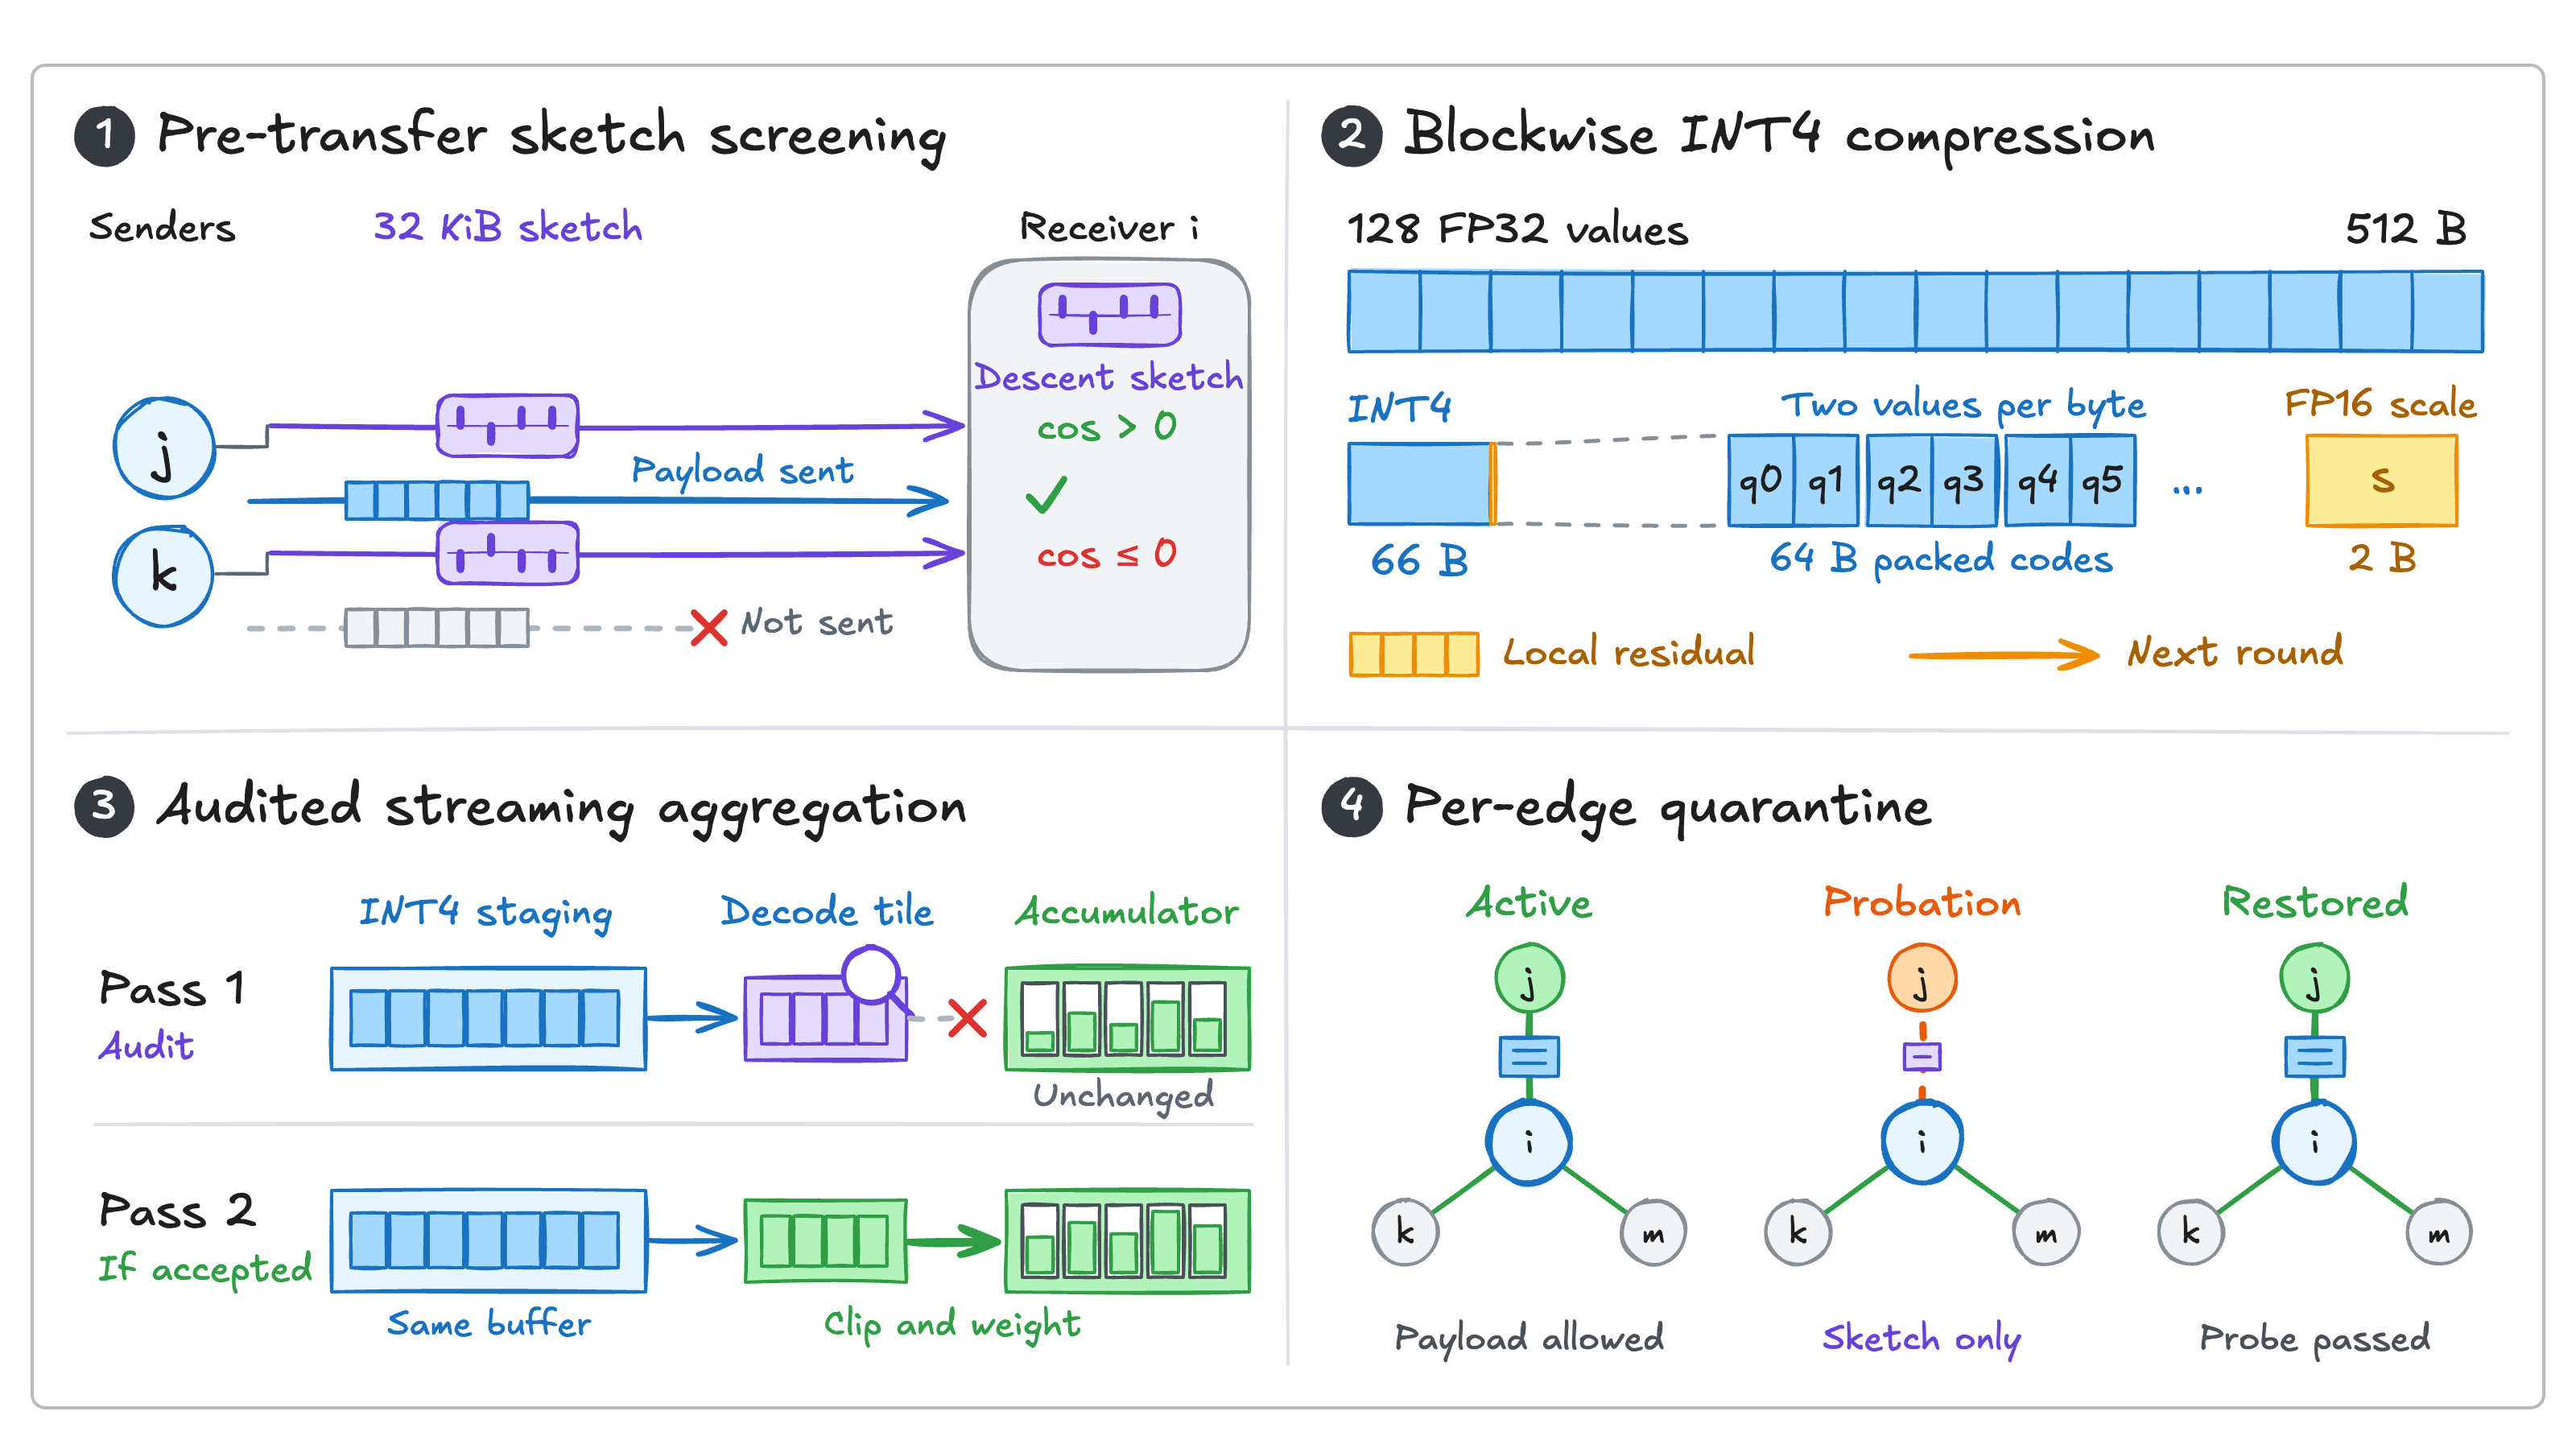
\includegraphics[width=\linewidth]{figures/fig1_story.png}
  \captionof{figure}{PeerSieve's four mechanisms: sketch screening, INT4 compression, audited streaming, and link quarantine.}
  \label{fig:story}
\end{inlinefigure}

We propose \textbf{PeerSieve} for decentralized large language model (LLM) fine-tuning. It separates the decision to request an update from the decision to aggregate it. The four mechanisms in Figure~\ref{fig:story} address the gaps in the same order:
\begin{enumerate}
  \item \textbf{Pre-transfer sketch screening.} The receiver compares CountSketch summaries~\cite{charikar2004countsketch,rothchild2020fetchsgd} of the decoded update and its own validation descent direction. It requests the payload only if the sketch cosine is positive. Passing the screen permits transfer, not aggregation.
  \item \textbf{Blockwise INT4 compression.} Before announcing the sketch, the sender quantizes the update in blocks and saves the residual for the next round. Each requested payload is 49.63~MiB instead of 385~MiB without selecting a sparse subset of coordinates. We will measure how quantization affects alignment on recorded updates.
  \item \textbf{Audited streaming aggregation.} The receiver reuses one compressed staging buffer and one decode tile. Pass~1 audits the payload. Only after it passes does Pass~2 cap its norm at the receiver's own update norm and add it to the accumulator. For fixed update and sketch sizes, receive-side tensor buffers do not grow with neighbor degree.
  \item \textbf{Per-edge quarantine.} Persistent misalignment or a soft audit failure puts an edge on probation. A passing sketch-only probe can restore it without a payload transfer. Hard protocol faults trigger a ban at that receiver for the rest of the run. Best-effort two-hop referrals can replenish the active neighbor set.
\end{enumerate}

We will test whether PeerSieve reduces received bytes, round time, and receive-side memory while preserving model quality and limiting the influence of Byzantine updates. We will first attempt to reproduce the TrustGraph-DFL baseline on CIFAR-10, then compare PeerSieve against baselines and ablations in a controlled language-model study (Section~\ref{sec:eval}).

\section{System Model and Design Invariants}
\label{sec:scope}

We consider synchronous instruction tuning of TinyLlama-1.1B~\cite{zhang2024tinyllama} on Dolly-15k~\cite{conover2023dolly}, using LoRA~\cite{hu2022lora} or full-parameter updates. Peers exchange messages through \texttt{torch.distributed} point-to-point communication. A token bucket emulates a shared receive budget at each peer. Authentication identifies the sender but does not establish how an update was produced. The adversarial degrees in Table~\ref{tab:scope} describe evaluation settings, not proven tolerance bounds.

\begin{table}[htbp]
  \caption{System scope, threat model, and assumptions about trusted state.}
  \label{tab:scope}
  \centering\small
  \begin{tabularx}{\linewidth}{@{}P{0.19\linewidth}Y@{}}
    \toprule
    Dimension & Scope \\
    \midrule
    Workload & TinyLlama-1.1B with rank-32 LoRA, rank-128 LoRA, or full-parameter tuning. Non-IID Dolly-15k data across eight peers in the main experiment and up to 16 in the degree sweep. \\
    Threat model & Up to two of six neighbors are Byzantine in the main setting and up to three in the stress setting. Each round's sketch seed is public. \\
    Trusted state & An honest receiver trusts its local training and validation data, random number generator, round counter, and transport state. Peer identities are fixed and authenticated for the run. \\
    Compression & Packed INT4 with one FP16 scale per 128-element block and a local FP32 error-feedback residual. \\
    Verification & A 32~KiB FP16 sketch screen followed by checks of payload format, sketch agreement, alignment, and norm. \\
    Edge policy & Reversible probation and best-effort two-hop referral when observed active degree falls below two. \\
    Exclusions & Asynchronous staleness, Sybil identities, corrupted local validation data, and hardware bit flips. The protocol does not guarantee connectivity of the honest subgraph. \\
    \bottomrule
  \end{tabularx}
\end{table}

Under these assumptions, the receiver is designed to enforce four invariants:

\textbf{I1 (audit before accumulation).} A received payload contributes to the running aggregate only after passing all audit checks. The audit checks consistency and alignment, not training provenance.

\textbf{I2 (degree-independent tensor buffers).} The receiver holds one compressed staging buffer, one dequantization tile, one validation vector, and one accumulator. For fixed trainable dimension and sketch size, these buffers are independent of degree. Per-edge metadata can still grow with degree.

\textbf{I3 (bounded staging on hard faults).} The receiver stages only requested, size-bounded payloads. After a hard protocol fault, it refuses further transfers from that sender for the rest of the run. This limits hard-failing payloads to one per sender at a given receiver, not all Byzantine traffic.

\textbf{I4 (reversible probation).} Low alignment or a soft audit failure can place an edge on probation rather than trigger a ban. Scheduled probes allow an eligible edge to return to active status.

\section{System Design}
\label{sec:design}

PeerSieve uses a compact sketch to decide whether to request an update and the decoded payload to decide whether to aggregate it. We first define the update representation, then describe the messages exchanged within each round and how screening and audit outcomes affect subsequent rounds.

\subsection{Notation and Blockwise Compression}

Let $d$ denote the trainable dimension and $K$ the receiver's neighbor degree. Index synchronous rounds by $t$. Peer $j$ trains locally and forms the parameter increment $\Delta w_j^{(t)} = w_j^{(t,\mathrm{after})} - w_j^{(t)}$. At the start of the round, receiver $i$ computes its validation descent direction $g_i^{\mathrm{val}} = -\nabla L_i^{\mathrm{val}}(w_i^{(t)})$. A positive dot product with this direction predicts a first-order decrease in validation loss, not necessarily a decrease after a finite step. The negative sign follows from defining the increment as after-minus-before.

The running example uses TinyLlama-1.1B with rank-128 LoRA on seven linear projections in each of 22 layers. The resulting $100{,}925{,}440$ trainable parameters occupy $385.0$~MiB in FP32. Peer $i$ has six neighbors, including two Byzantine peers in the illustration, and a shared receive budget of $1$~Gb/s.

\begin{inlinefigure}
  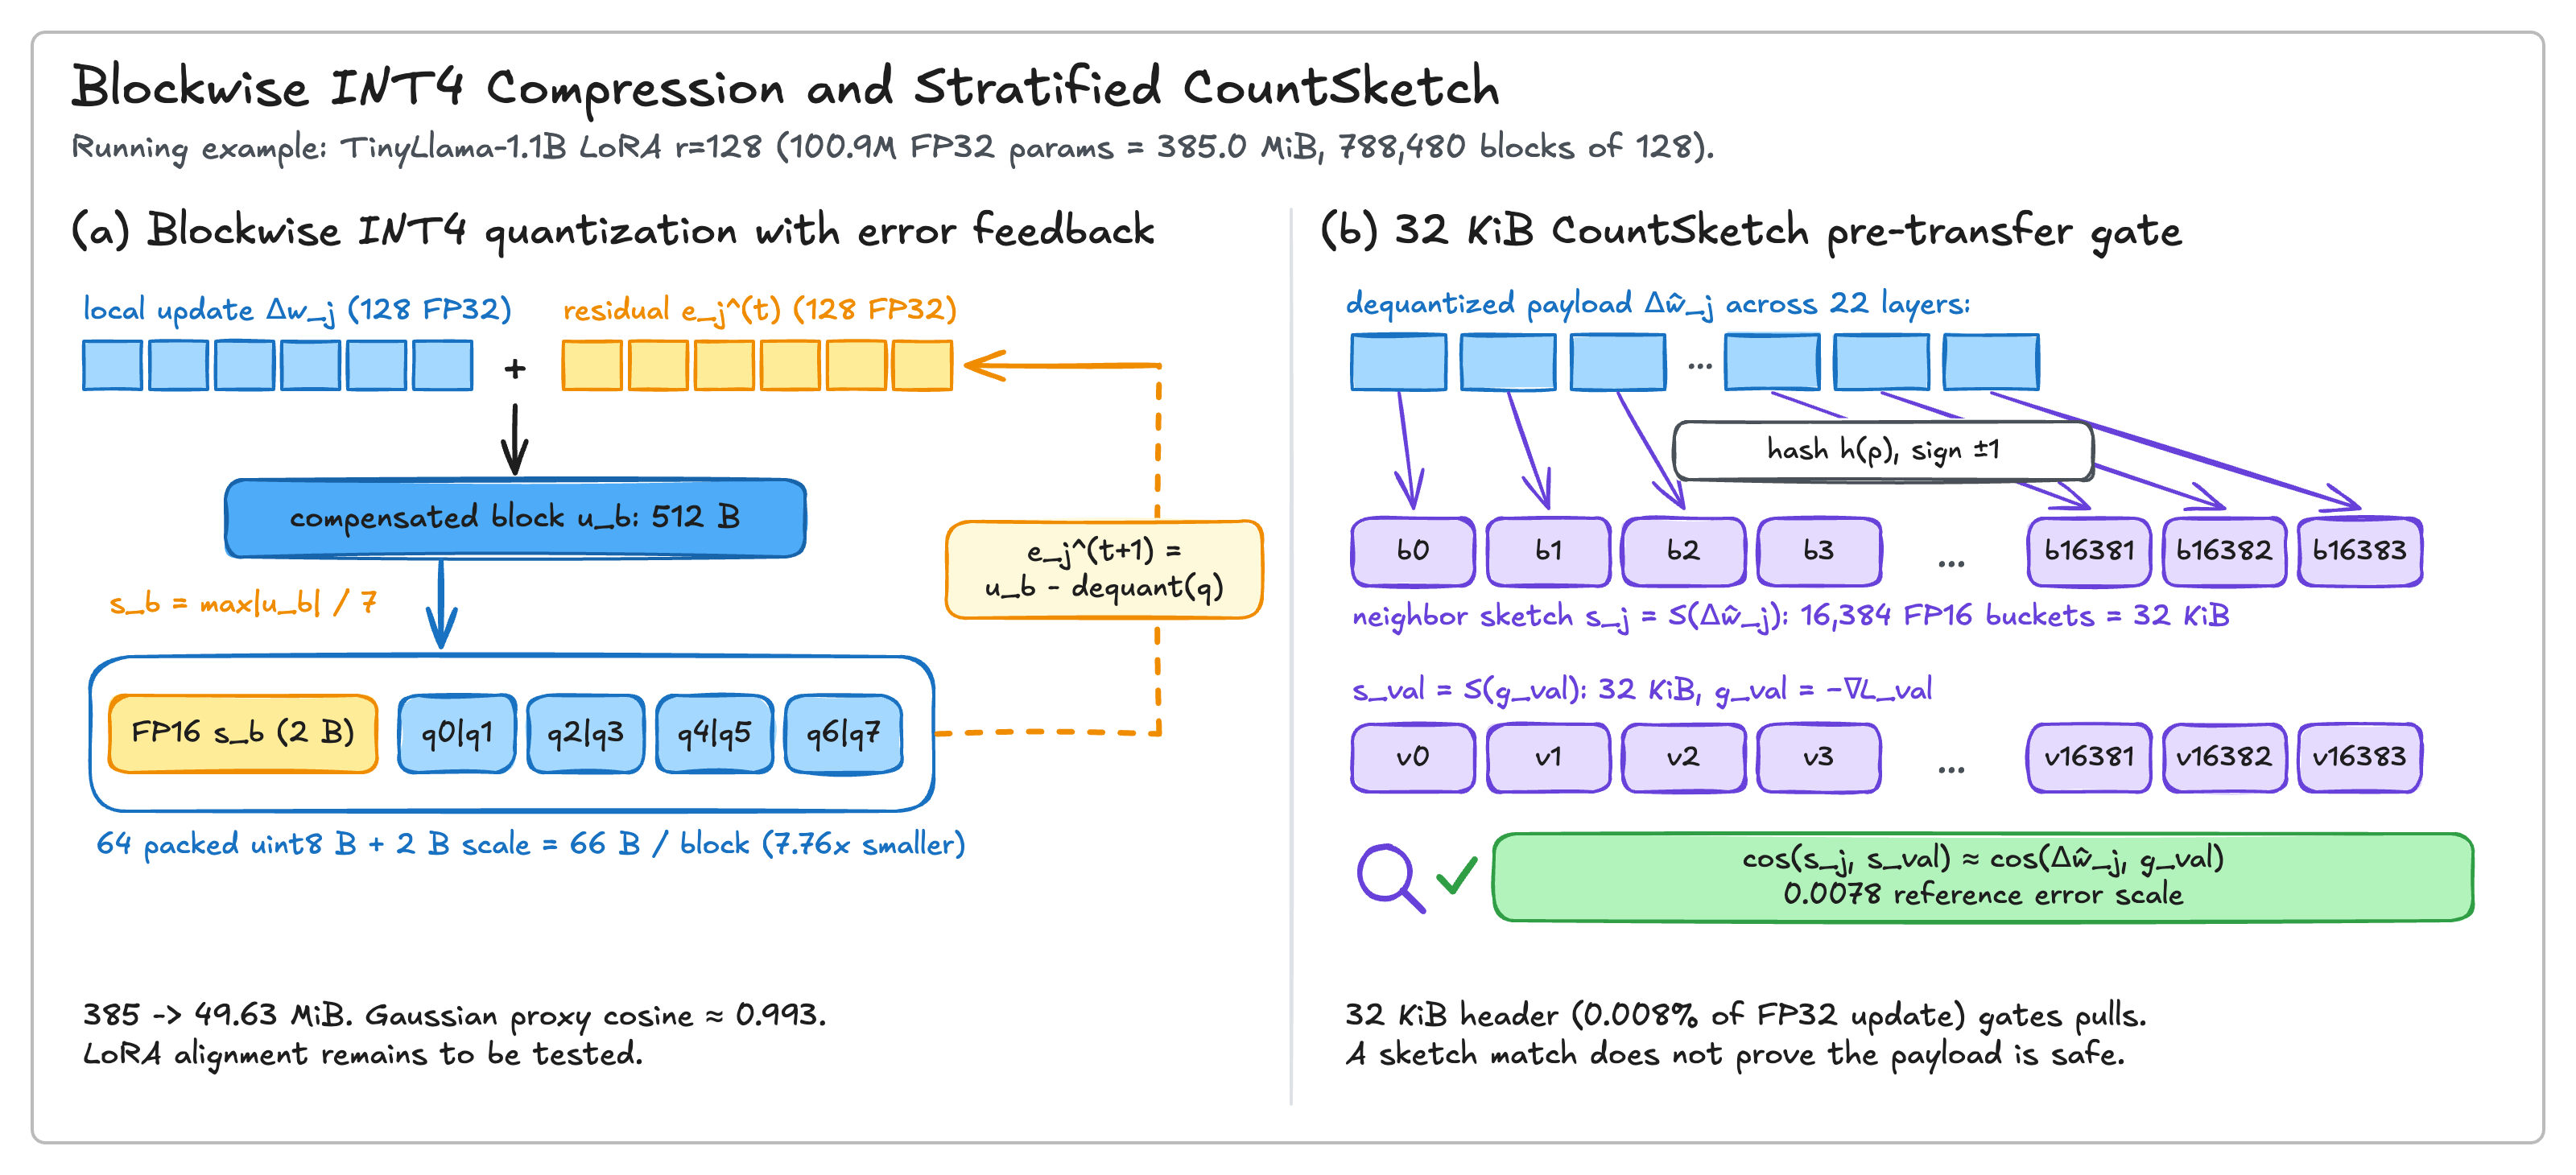
\includegraphics[width=\linewidth]{figures/fig2_compress.png}
  \captionof{figure}{Blockwise encoding uses 64 packed INT4 bytes and a two-byte FP16 scale per 128-element block, a $7.76\times$ reduction relative to FP32. Sketching the decoded update lets the receiver reproduce the announcement during the payload audit.}
  \label{fig:compress}
\end{inlinefigure}

Blockwise INT4 reduces the size of each payload that passes the sketch screen. The sender partitions the increment into 128-element blocks ($788{,}480$ in the running example), adds its previous FP32 residual, and applies Equation~\eqref{eq:quant}. The scale $s_b$ is the largest absolute entry of the residual-corrected block divided by seven, rounded to the transmitted FP16 format. The sender uses this rounded scale both to reconstruct the block and to compute the next residual. A zero scale encodes an all-zero decoded block.
\begin{equation}
\begin{aligned}
  u_{j,b}^{(t)} &= \Delta w_{j,b}^{(t)} + e_{j,b}^{(t)}, \\
  q_{j,b}^{(t)} &= \operatorname{clip}\!\left(\operatorname{round}\!\left(u_{j,b}^{(t)}/s_b\right),-7,7\right),
                   \qquad s_b>0, \\
  y_{j,b}^{(t)} &= s_b q_{j,b}^{(t)}, \qquad
  e_{j,b}^{(t+1)} = u_{j,b}^{(t)} - y_{j,b}^{(t)} .
\end{aligned}
\label{eq:quant}
\end{equation}

The sender reconstructs the same vector $y_j^{(t)}$ as the receiver (denoted $\widehat{\Delta w}_j^{(t)}$ in Figure~\ref{fig:compress}). An encoded block occupies 66~B rather than 512~B in FP32, yielding a 49.63~MiB payload in the running example. The mean cosine between input and decoded blocks was approximately $0.993$ in a synthetic Gaussian-block check. Alignment on recorded LoRA updates remains to be measured. Error feedback carries quantization residuals into the next local update. It does not compensate for rejection or receiver-side clipping.

\subsection{Sketch Screen}

The sketch screen estimates how well the decoded update aligns with the receiver's validation descent direction without transferring the full payload. The ideal CountSketch $\mathcal S_t$ assigns each coordinate to a bucket with a sign. It allocates $m=16{,}384$ buckets across layers in proportion to their parameter counts. Peers share the hashes and signs for the round. We write $F_t(v)$ for the canonical sketch obtained by accumulating the signed coordinates of $v$ in FP32 in a fixed reduction order and rounding the resulting buckets to FP16. The wire format excludes nonfinite values and uses one representation for zero. Sender $j$ announces $s_j^{(t)}=F_t(y_j^{(t)})$, and receiver $i$ computes $s_i^{\mathrm{val}}=F_t(g_i^{\mathrm{val}})$. Using the same decoding and reduction order lets the receiver reproduce the announcement for a valid payload. Equation~\eqref{eq:sketch} distinguishes the sketch cosine from the full-vector cosine used in the payload audit.
\begin{equation}
\begin{aligned}
  \widehat c_{ij}^{(t)} &=\frac{\langle s_j^{(t)},s_i^{\mathrm{val}}\rangle}
  {\|s_j^{(t)}\|_2\|s_i^{\mathrm{val}}\|_2}, &
  c_{ij}^{(t)} &=\frac{\langle y_j^{(t)},g_i^{\mathrm{val}}\rangle}
  {\|y_j^{(t)}\|_2\|g_i^{\mathrm{val}}\|_2} .
\end{aligned}
\label{eq:sketch}
\end{equation}

The receiver skips comparisons with zero norms. An FP16 sketch occupies 32~KiB, about $0.008\%$ of the FP32 rank-128 update. Under independent signed hashing, the ideal sketch gives an unbiased inner-product estimate for inputs fixed independently of the hashes and signs. This does not imply that the sketch cosine, which divides by random norms, is unbiased. The scale $m^{-1/2}\approx 0.0078$ is a heuristic, not a tail bound for the layer-partitioned FP16 sketch. We will measure tail errors on recorded updates.

\subsection{Two-Phase Round Protocol}

\begin{inlinefigure}
  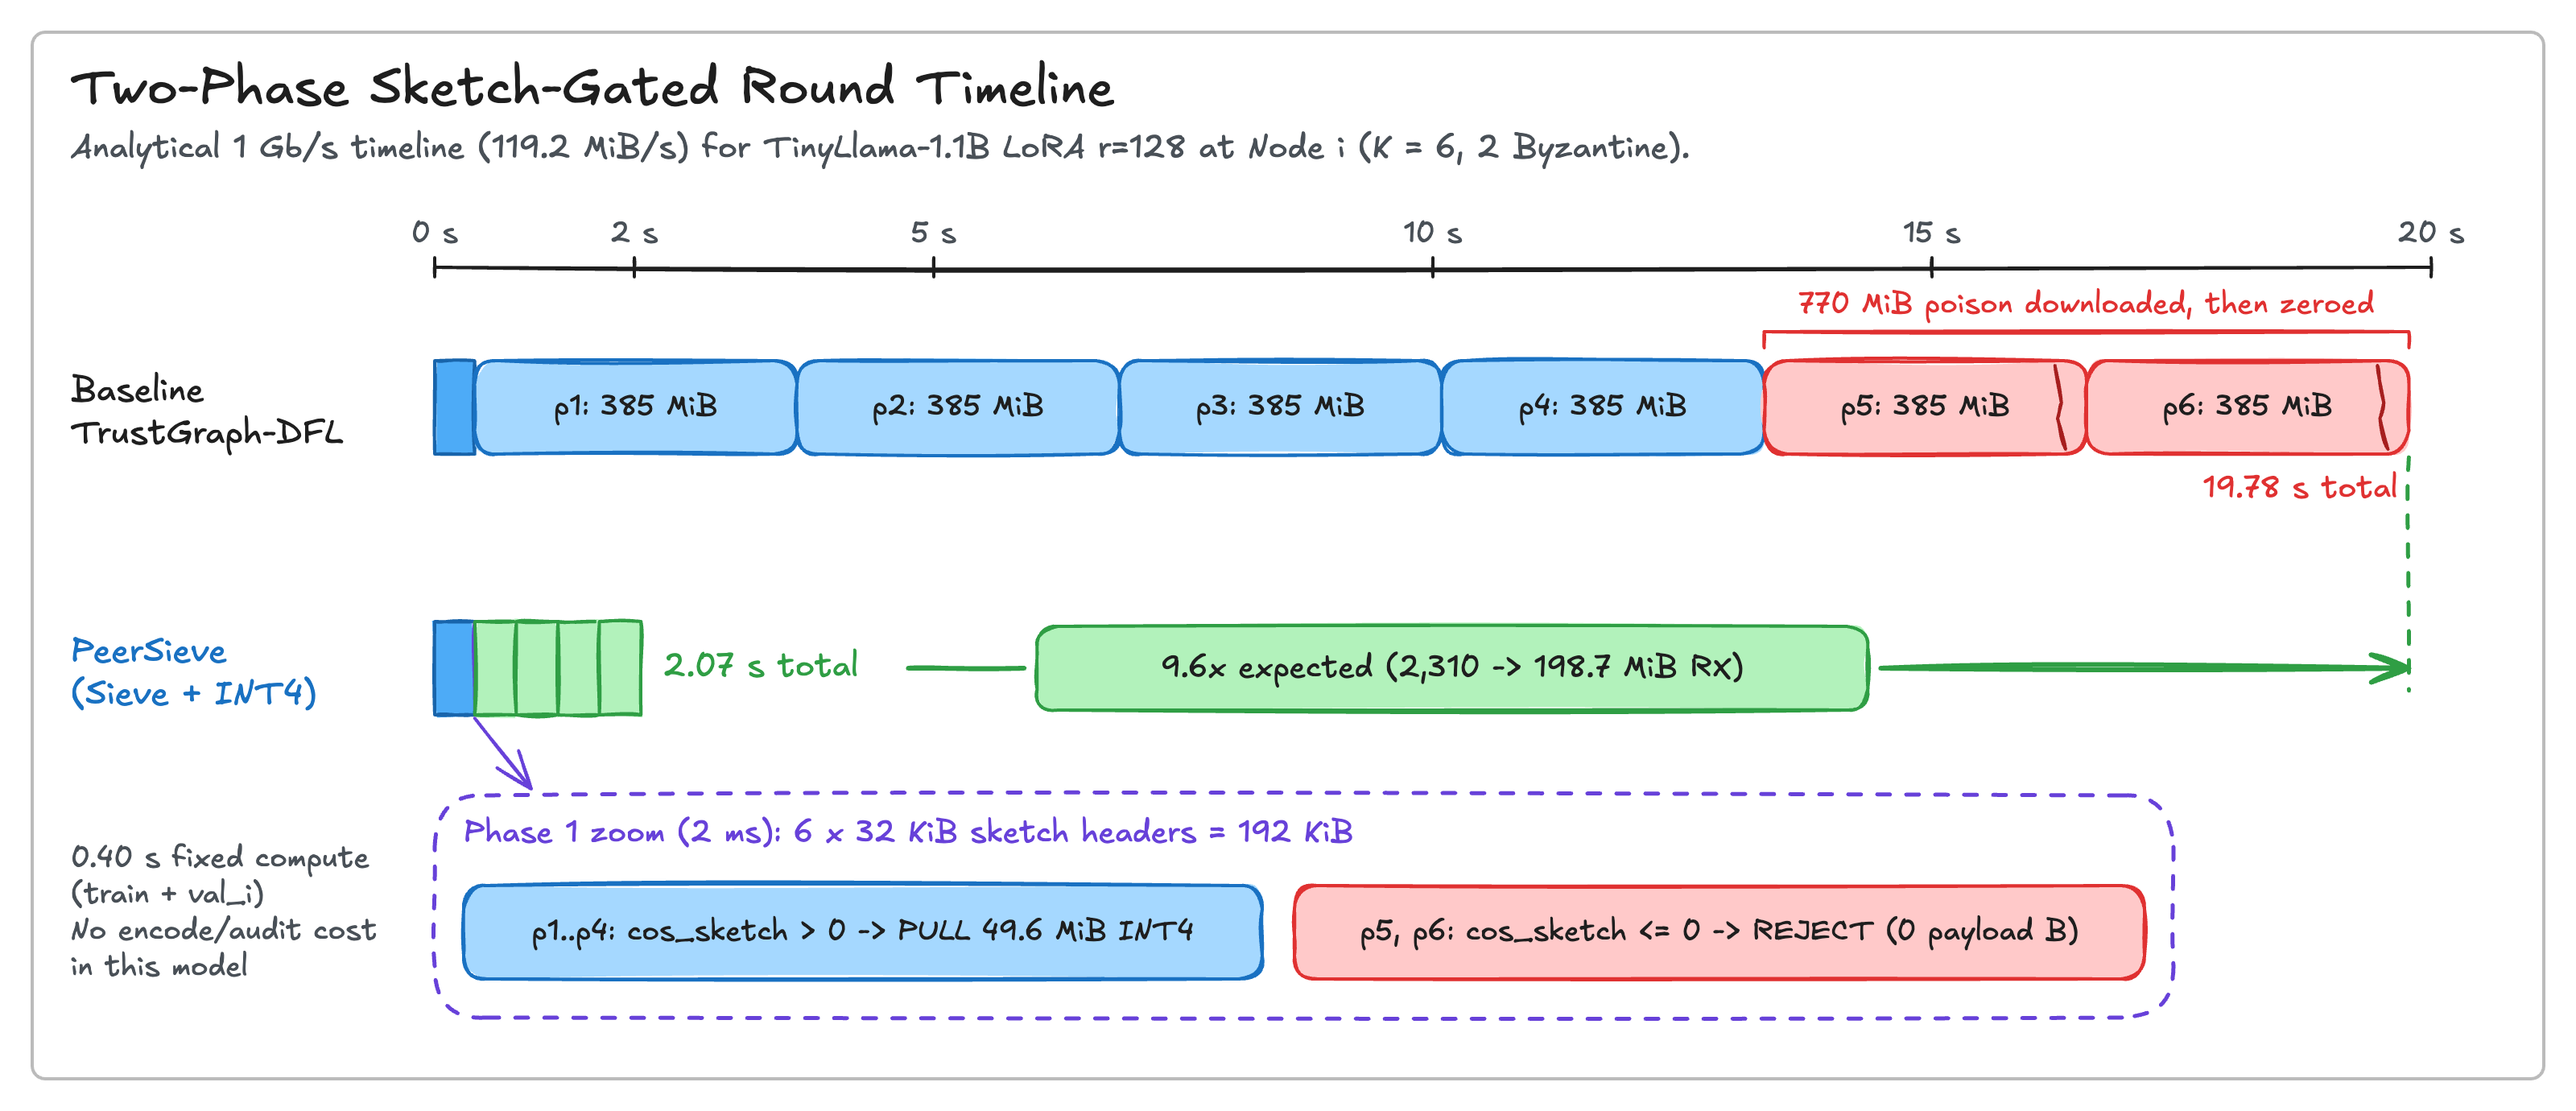
\includegraphics[width=\linewidth]{figures/fig3_protocol.png}
  \captionof{figure}{Modeled round at $1$~Gb/s. The FP32 baseline spends 19.38~s receiving six updates. PeerSieve receives six sketches and four 49.63~MiB payloads. The totals include 0.40~s of local computation but exclude encoding, auditing, and transport overhead.}
  \label{fig:protocol}
\end{inlinefigure}

The two phases in Figure~\ref{fig:protocol} specify what peers exchange over the network: first sketches, then requested payloads. The two passes in Section~\ref{sec:audit} are local operations on a staged payload in the second phase. Passing the sketch screen permits transfer, not accumulation.

\begin{enumerate}
  \item \textbf{Local preparation.} Peer $i$ computes its validation descent direction and sketch, runs four local optimizer steps, and encodes and sketches its increment.
  \item \textbf{Phase 1: Announce and screen.} Each active peer sends a fixed-size announcement bound to its authenticated identity, run, and round. Six sketch bodies total 192~KiB (about 1.6~ms at $1$~Gb/s). The receiver requests a payload only if the sketch cosine in Equation~\eqref{eq:sketch} is strictly positive. Probation probes follow Section~\ref{sec:quarantine}.
  \item \textbf{Phase 2: Transfer and process requested payloads.} Each request authorizes one size-bounded transfer from that peer in the current round. The receiver stages one payload at a time, audits it in the first pass, and accumulates its contribution in the second pass only on acceptance.
  \item \textbf{Round completion.} The receiver normalizes the accumulated neighbor update once and updates the edge states.
\end{enumerate}

Table~\ref{tab:round} assumes serial reception under the shared bandwidth budget. Before quarantine, the sketch screen rejects two of the six neighbors. The four-active-edge case assumes that all remaining peers pass the screen and no probation probes are due. The two cases differ only in sketch traffic.

\begin{table}[htbp]
  \caption{Modeled per-receiver costs for rank-128 LoRA at initial degree six. RX VRAM counts receive-side tensor buffers, not total training memory. The Top-1\% row assumes 8~B per nonzero and dense buffers after expansion.}
  \label{tab:round}
  \centering\small
  \begin{tabularx}{\linewidth}{@{}Yrrr@{}}
    \toprule
    Configuration & RX (MiB) & RX + compute (s) & RX VRAM (MiB) \\
    \midrule
    Batched TrustGraph-DFL (FP32) & 2,310.0 & 19.78 & 3,080.0 \\
    Sparse Top-1\% + TrustGraph & 46.2 & Not modeled & 3,080.0 \\
    Blockwise INT4, no sketch screen & 297.8 & 2.90 & 3,080.0 \\
    PeerSieve, sketch screen before quarantine & 198.7 & 2.07 & 823.6 \\
    PeerSieve, four active edges & 198.6 & 2.07 & 823.6 \\
    \bottomrule
  \end{tabularx}
\end{table}

\subsection{Payload Audit and Streaming Aggregation}
\label{sec:audit}

The sketch screen does not establish full-vector alignment or bound update magnitude. In exact arithmetic, multiplying an update and its announcement by the same positive factor leaves both cosine scores and the sketch-to-payload norm ratio unchanged. The receiver therefore checks the decoded update before accumulation and caps its norm before adding it. Inspired by FLTrust's magnitude normalization~\cite{cao2021fltrust}, the cap leaves small updates unchanged rather than scaling them up. The cap is $r_i^{(t)}=\|\Delta w_i^{(t)}\|_2$, the norm of the receiver's own unclipped, uncompressed increment. The receiver computes this scalar locally without relying on a sender-reported norm. Let $\mathcal N_i^{\mathrm{acc}}$ denote the neighbors whose nonzero payloads pass the audit. Equation~\eqref{eq:stream} defines the clipping factor, trust weight, and neighbor aggregate. The aggregate is defined only when the total trust weight is positive.
\begin{equation}
\begin{aligned}
  a_{ij}^{(t)} &= \min\!\left(1,\frac{r_i^{(t)}}{\|y_j^{(t)}\|_2}\right), \qquad
  \widetilde w_{ij}^{(t)} = \max\!\left(0,c_{ij}^{(t)}\right), \\
  W_i^{(t)} &= \sum_{j\in\mathcal N_i^{\mathrm{acc}}} \widetilde w_{ij}^{(t)}, \qquad
  \Delta\bar w_i^{(t)} = \frac{1}{W_i^{(t)}}
  \sum_{j\in\mathcal N_i^{\mathrm{acc}}}\widetilde w_{ij}^{(t)} a_{ij}^{(t)} y_j^{(t)} .
\end{aligned}
\label{eq:stream}
\end{equation}
The denominator sums the trust weights, not the clipping factors. For $W_i^{(t)}>0$, the triangle inequality gives $\|\Delta\bar w_i^{(t)}\|_2\le r_i^{(t)}$. This bounds the magnitude of the neighbor increment, not the fraction of trust assigned to a Byzantine peer. In the planned LLM experiments, we blend the local and neighbor increments with self-weight $0.5$. If $W_i^{(t)}=0$, the receiver keeps its locally trained model without a neighbor step.

\begin{inlinefigure}
  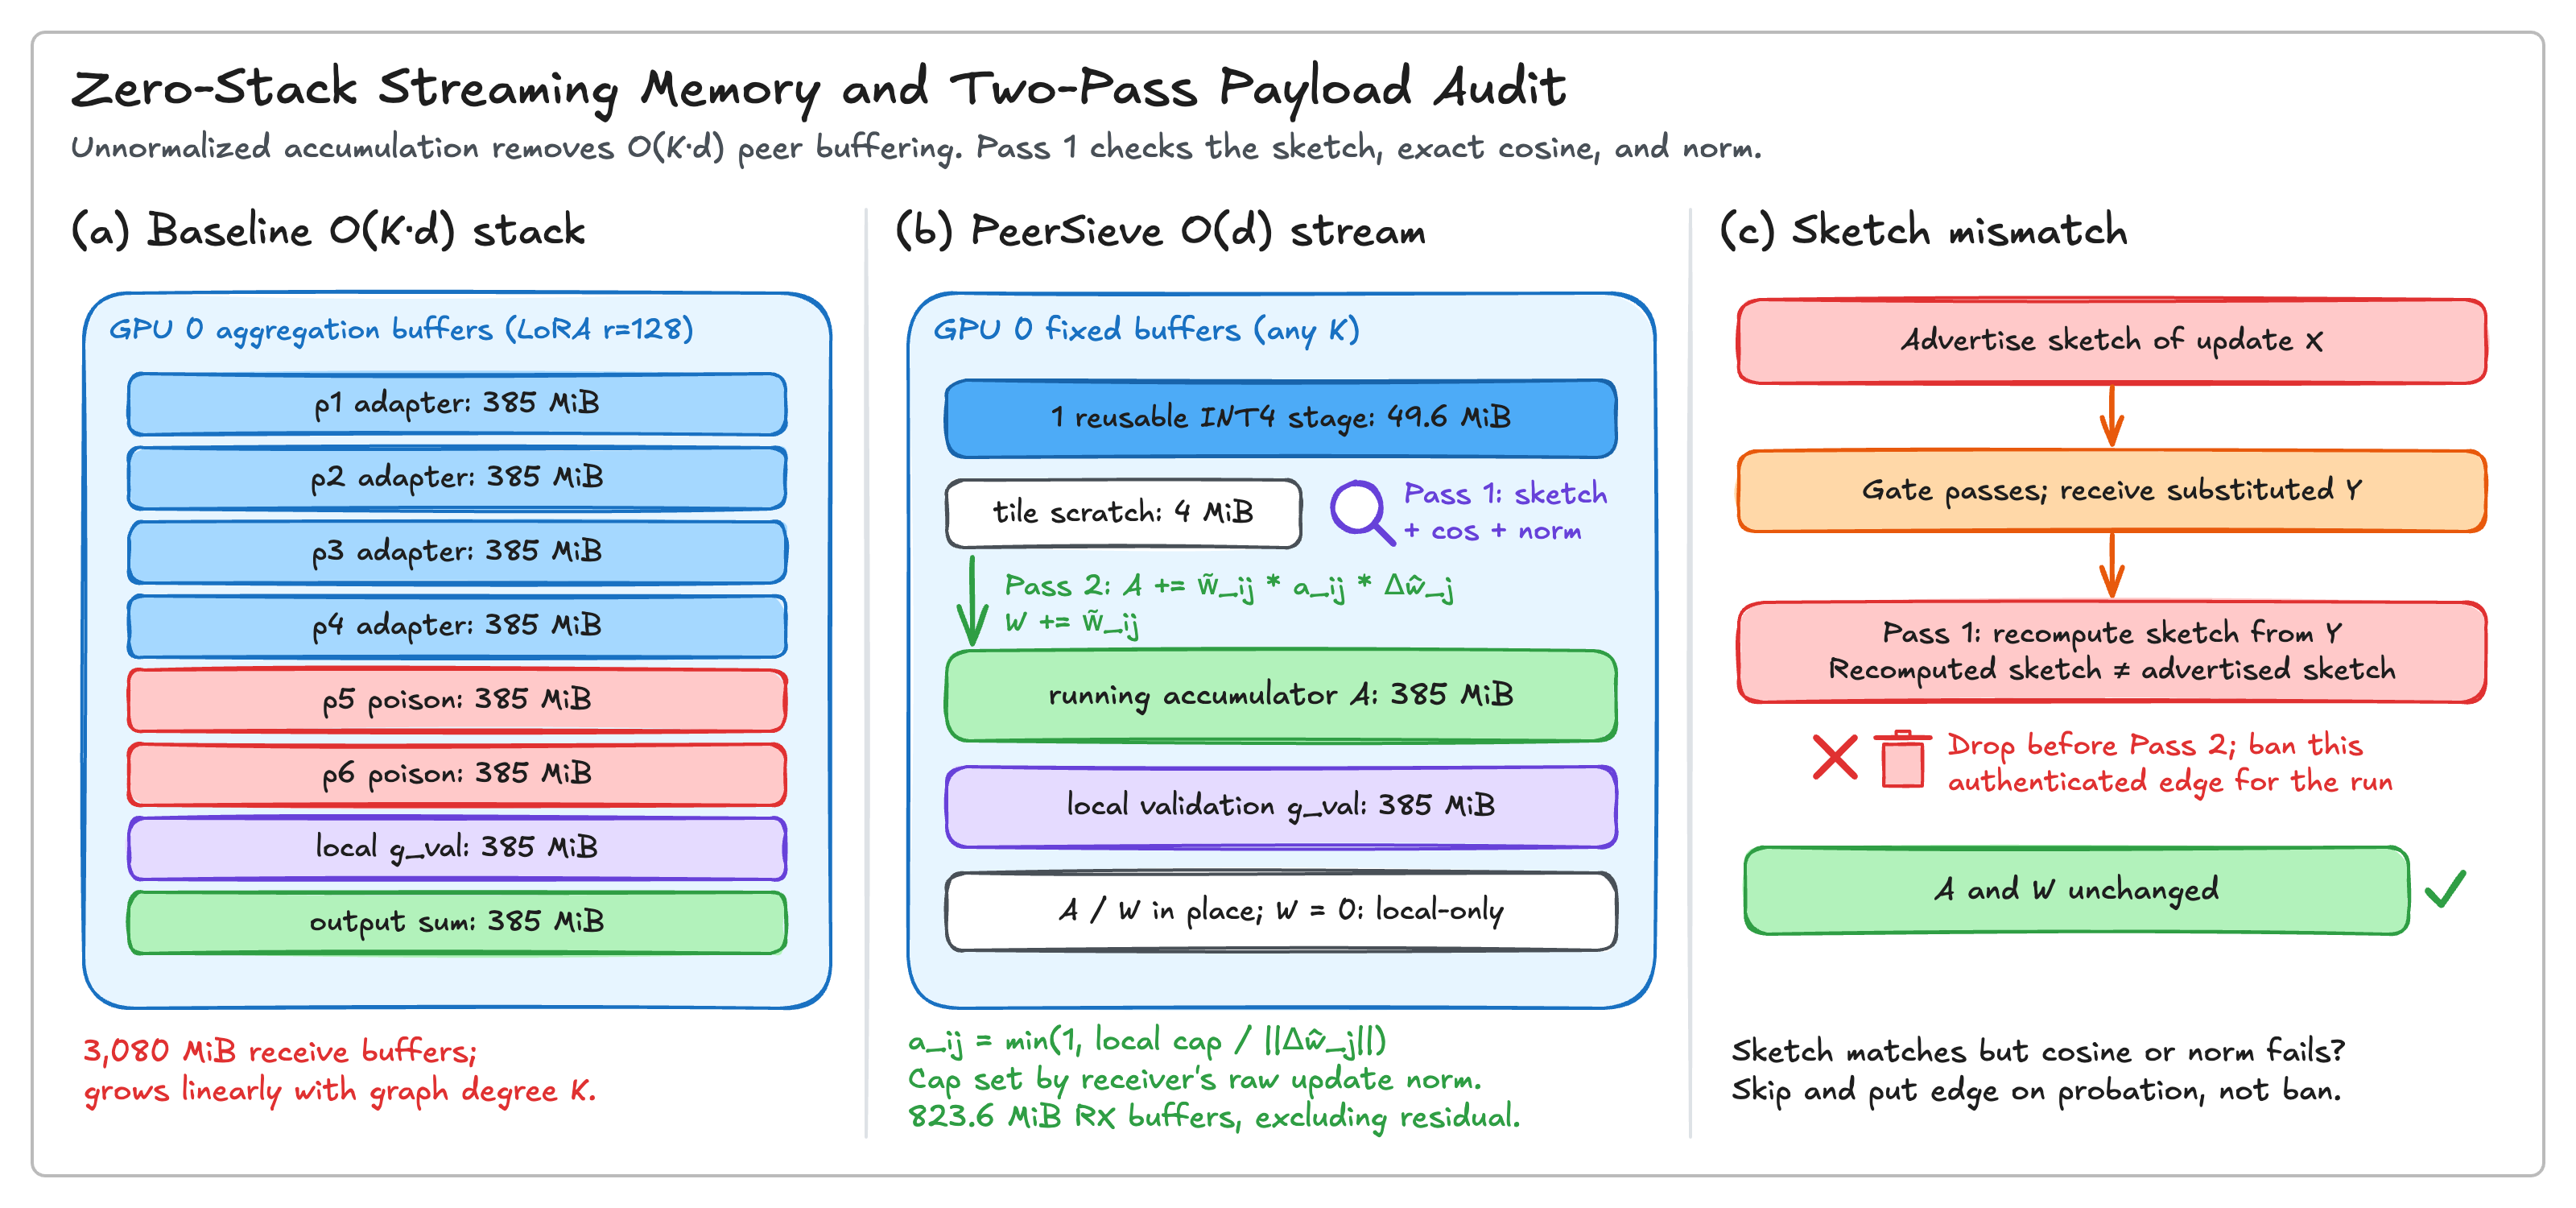
\includegraphics[width=\linewidth]{figures/fig4_stream.png}
  \captionof{figure}{Receive-side tensor buffers for batched and streaming aggregation. The batched baseline holds one dense buffer per neighbor. PeerSieve reuses one compressed staging buffer and one decode tile. Pass~1 performs the payload audit without changing the accumulator. Pass~2 adds the clipped, trust-weighted update only if the audit passes.}
  \label{fig:stream}
\end{inlinefigure}

\textbf{Pass 1: Audit without accumulation.} The receiver checks the sender identity, round, payload length, and packed format, then decodes the payload in tiles of at most 4~MiB. It recomputes the canonical sketch $F_t(y_j^{(t)})$ and calculates the full-vector cosine $c_{ij}^{(t)}$ and the norm $\|y_j^{(t)}\|_2$. For well-formed, finite, nonzero inputs, all four conditions must hold:
\begin{equation}
\begin{aligned}
  F_t(y_j^{(t)}) &= s_j^{(t)}, & c_{ij}^{(t)} &> 0, \\
  |\widehat c_{ij}^{(t)}-c_{ij}^{(t)}| &\le \tau_c, &
  \left|\frac{\|s_j^{(t)}\|_2}{\|y_j^{(t)}\|_2}-1\right| &\le \tau_n .
\end{aligned}
\label{eq:audit}
\end{equation}
The initial tolerances are $\tau_c=0.05$ and $\tau_n=0.03$. We will recalibrate them using empirical $99.9$th-percentile discrepancies from separate attack-free runs and freeze them before evaluation. A malformed encoding or a conflicting canonical sketch is a protocol fault that warrants a ban on that edge for the rest of the run. Finite alignment or norm disagreement is a soft failure. The receiver discards the staged payload and puts the edge on probation. It can skip a zero update without a hard ban.

\textbf{Pass 2: Accumulate accepted payloads.} The receiver reads the same unchanged staging buffer and adds $\widetilde w_{ij}^{(t)} a_{ij}^{(t)}y_j^{(t)}$ tile by tile. Only an accepted payload changes the accumulator or $W_i^{(t)}$. At round end the receiver divides the numerator in place if $W_i^{(t)}>0$. Reusing the staging buffer and tile avoids storing a dense copy for every neighbor. Figure~\ref{fig:stream} illustrates the receive-side tensor buffers for fixed $d$ and sketch size.

\textbf{Limits of the payload audit.} The equality check detects changes that alter the canonical sketch. A perturbation in the ideal sketch's nullspace leaves that sketch unchanged. If it also preserves the norm and validation alignment, the resulting payload can pass the audit, subject to finite-precision effects. In particular, a small norm discrepancy does not imply that the perturbation is small. The evaluation will measure how often such payloads pass and how they affect training.

\subsection{Link Quarantine and Topology Repair}
\label{sec:quarantine}

\begin{inlinefigure}
  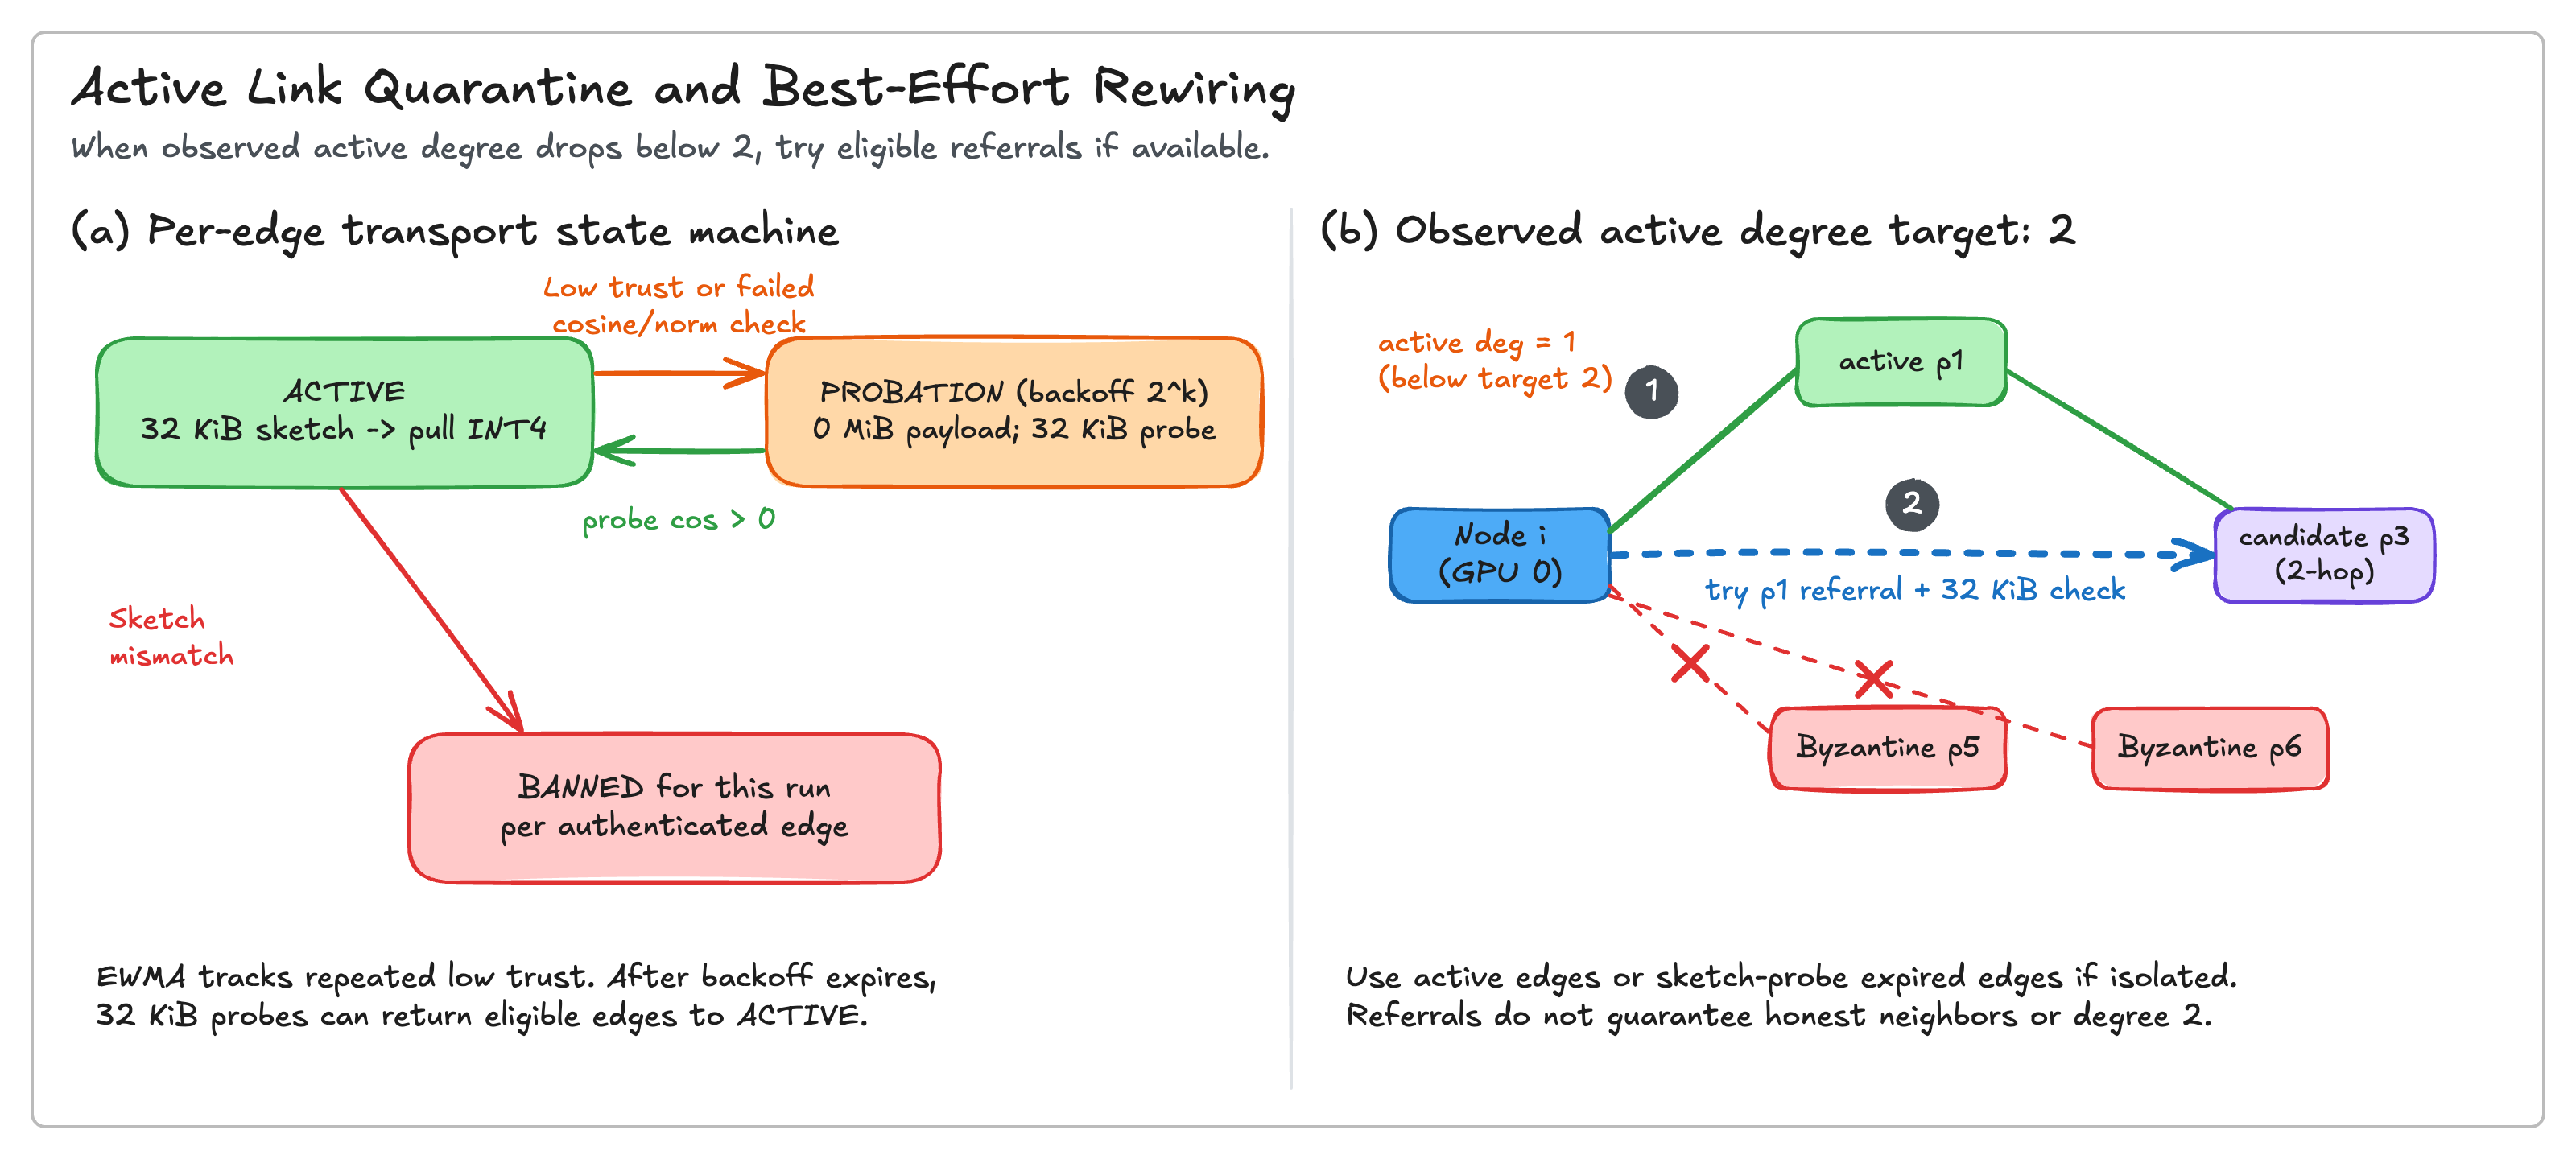
\includegraphics[width=\linewidth]{figures/fig5_quarantine.png}
  \captionof{figure}{Per-edge state transitions and an example of a successful two-hop referral. The repair target is an observed active neighbor degree of two. Reaching it depends on candidate reachability and the sketch screen.}
  \label{fig:quarantine}
\end{inlinefigure}

A single negative sketch score prevents a payload request but does not establish poisoning. To respond to persistent misalignment, the receiver keeps an exponentially weighted moving average (EWMA) of sketch scores for each edge. Figure~\ref{fig:quarantine} shows how an edge enters and leaves probation. An edge enters probation after three consecutive rounds with $R_{ij}^{(t)}<0$ or after a soft failure in the payload audit. The smoothing factor is $\beta=0.7$. The $k$th probation follows the backoff below, capped at $T_{\max}=16$ rounds.
\begin{equation}
  R_{ij}^{(t)}=\beta R_{ij}^{(t-1)}+(1-\beta)\widehat c_{ij}^{(t)}, \qquad
  T_{\mathrm{backoff}}(k)=\min\!\left(2^k,T_{\max}\right) .
\label{eq:backoff}
\end{equation}

\begin{inlinefigure}
  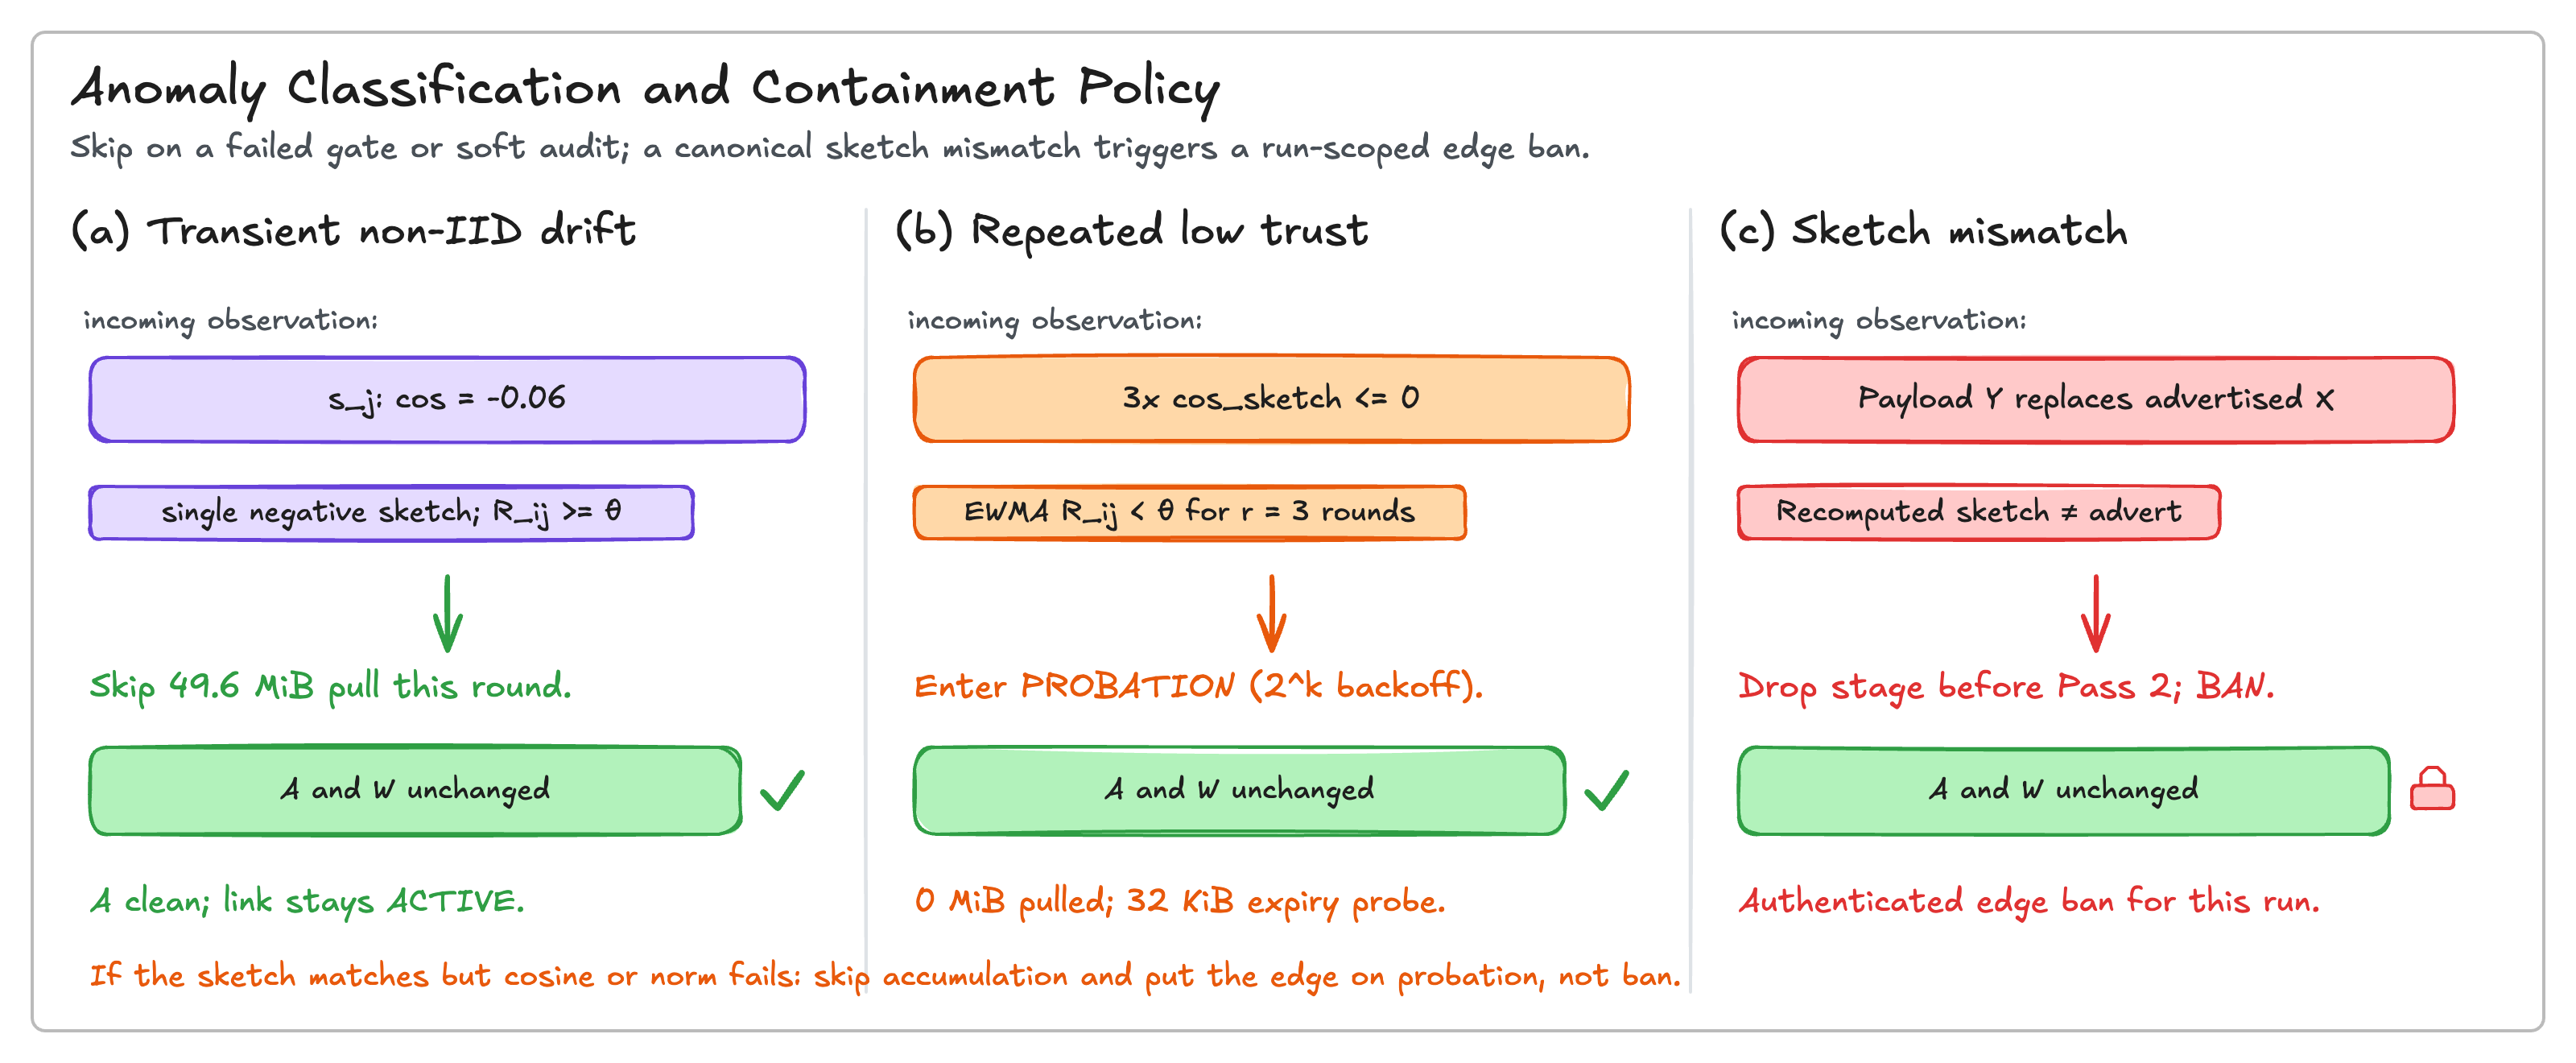
\includegraphics[width=\linewidth]{figures/fig6_policy.png}
  \captionof{figure}{Containment policy. Transient sketch misalignment skips the payload request. Persistent misalignment or a soft failure in the payload audit leads to probation. A hard protocol fault, such as a conflicting canonical sketch, leads to a ban. Rejected payloads never change the accumulator.}
  \label{fig:policy}
\end{inlinefigure}

Figure~\ref{fig:policy} links screening and audit outcomes to edge states. An edge on probation carries no payload. When probation expires, a 32~KiB probe that passes the sketch screen restores the edge to active status. A failed probe extends probation. In contrast, a hard protocol fault blocks further traffic from the peer at this receiver for the rest of the run.

Quarantine can lower the active neighbor degree. If the observed active neighbor degree drops below two, the receiver asks active neighbors for referrals and screens a sketch from an eligible, authenticated candidate. Rewiring respects the initial neighbor degree cap and never reinstates a banned peer. An isolated peer can still use scheduled probes on probation edges. Repair is best effort: it requires a reachable candidate, cannot identify which active peers are honest, and does not guarantee that the honest graph remains connected.

The checks in Table~\ref{tab:modules} must pass before GPU evaluation.

\begin{table}[htbp]
  \caption{Implementation modules and checks required before GPU evaluation.}
  \label{tab:modules}
  \centering\small
  \begin{tabularx}{\linewidth}{@{}P{0.23\linewidth}Y Y@{}}
    \toprule
    Module & Mechanism & Verification gate \\
    \midrule
    Blockwise INT4 + error feedback & 128-element packer and FP32 residual. & Check decoded values and residual accounting to floating-point tolerance. Measure cosine on recorded LoRA updates. \\
    Sketch screen & Layer-stratified CountSketch with deterministic FP32 reduction and FP16 wire format. & Check sender and receiver agreement across tiling. Measure cosine and norm error on attack-free traces. \\
    Payload audit and streaming aggregation & Reusable compressed staging buffer, tiled decoding, and scalar norm cap. & Verify that failed payload audits leave the accumulator and total weight unchanged and accepted updates respect the cap. \\
    Quarantine and referral & Authenticated edge states and capped backoff. & Use multi-process Gloo tests for hard-fault bans, soft-fault recovery, and reachability with and without eligible referrals. \\
    \bottomrule
  \end{tabularx}
\end{table}

\section{Evaluation Plan}
\label{sec:eval}

We propose two stages: a CIFAR-10 reproduction to establish a reference implementation, followed by a controlled study of language-model fine-tuning. The following questions guide the comparisons in the second stage.

\subsection{Research Questions}

\begin{enumerate}[label=\textbf{RQ\arabic*.}]
  \item \textbf{Model quality.} How does PeerSieve compare with FP32 TrustGraph-DFL in held-out perplexity and next-token accuracy under attack?
  \item \textbf{Robustness.} Which Byzantine updates pass screening and audit, what share of the aggregate trust weight do they receive, and how often are honest updates rejected?
  \item \textbf{Communication and time.} How do received bytes and round time vary with the receive-rate limit and with individual mechanisms enabled or disabled?
  \item \textbf{Memory.} Are receive-side tensor buffers independent of neighbor degree in practice, and can full-parameter tuning complete on one 40~GB A100 per peer?
\end{enumerate}

\subsection{Stage 1: CIFAR-10 Baseline Reproduction}

We will reimplement the TrustGraph-DFL preprint's 20-peer CNN experiment~\cite{trustgraph2026}. We will compare test accuracy with BALANCE at $30\%$ Byzantine peers and compare honest rejection rates with Krum in the $50\%$ stress setting. As printed, Algorithm~1 pairs an after-minus-before update with the positive validation loss gradient. We will test both the printed rule and the validation descent convention from Section~\ref{sec:design} and report agreement or discrepancies with the preprint. Stage~2 will use the descent-corrected FP32 implementation as its baseline, regardless of whether either convention reproduces the reported results.

\subsection{Stage 2: Language-Model Evaluation}

\begin{inlinefigure}
  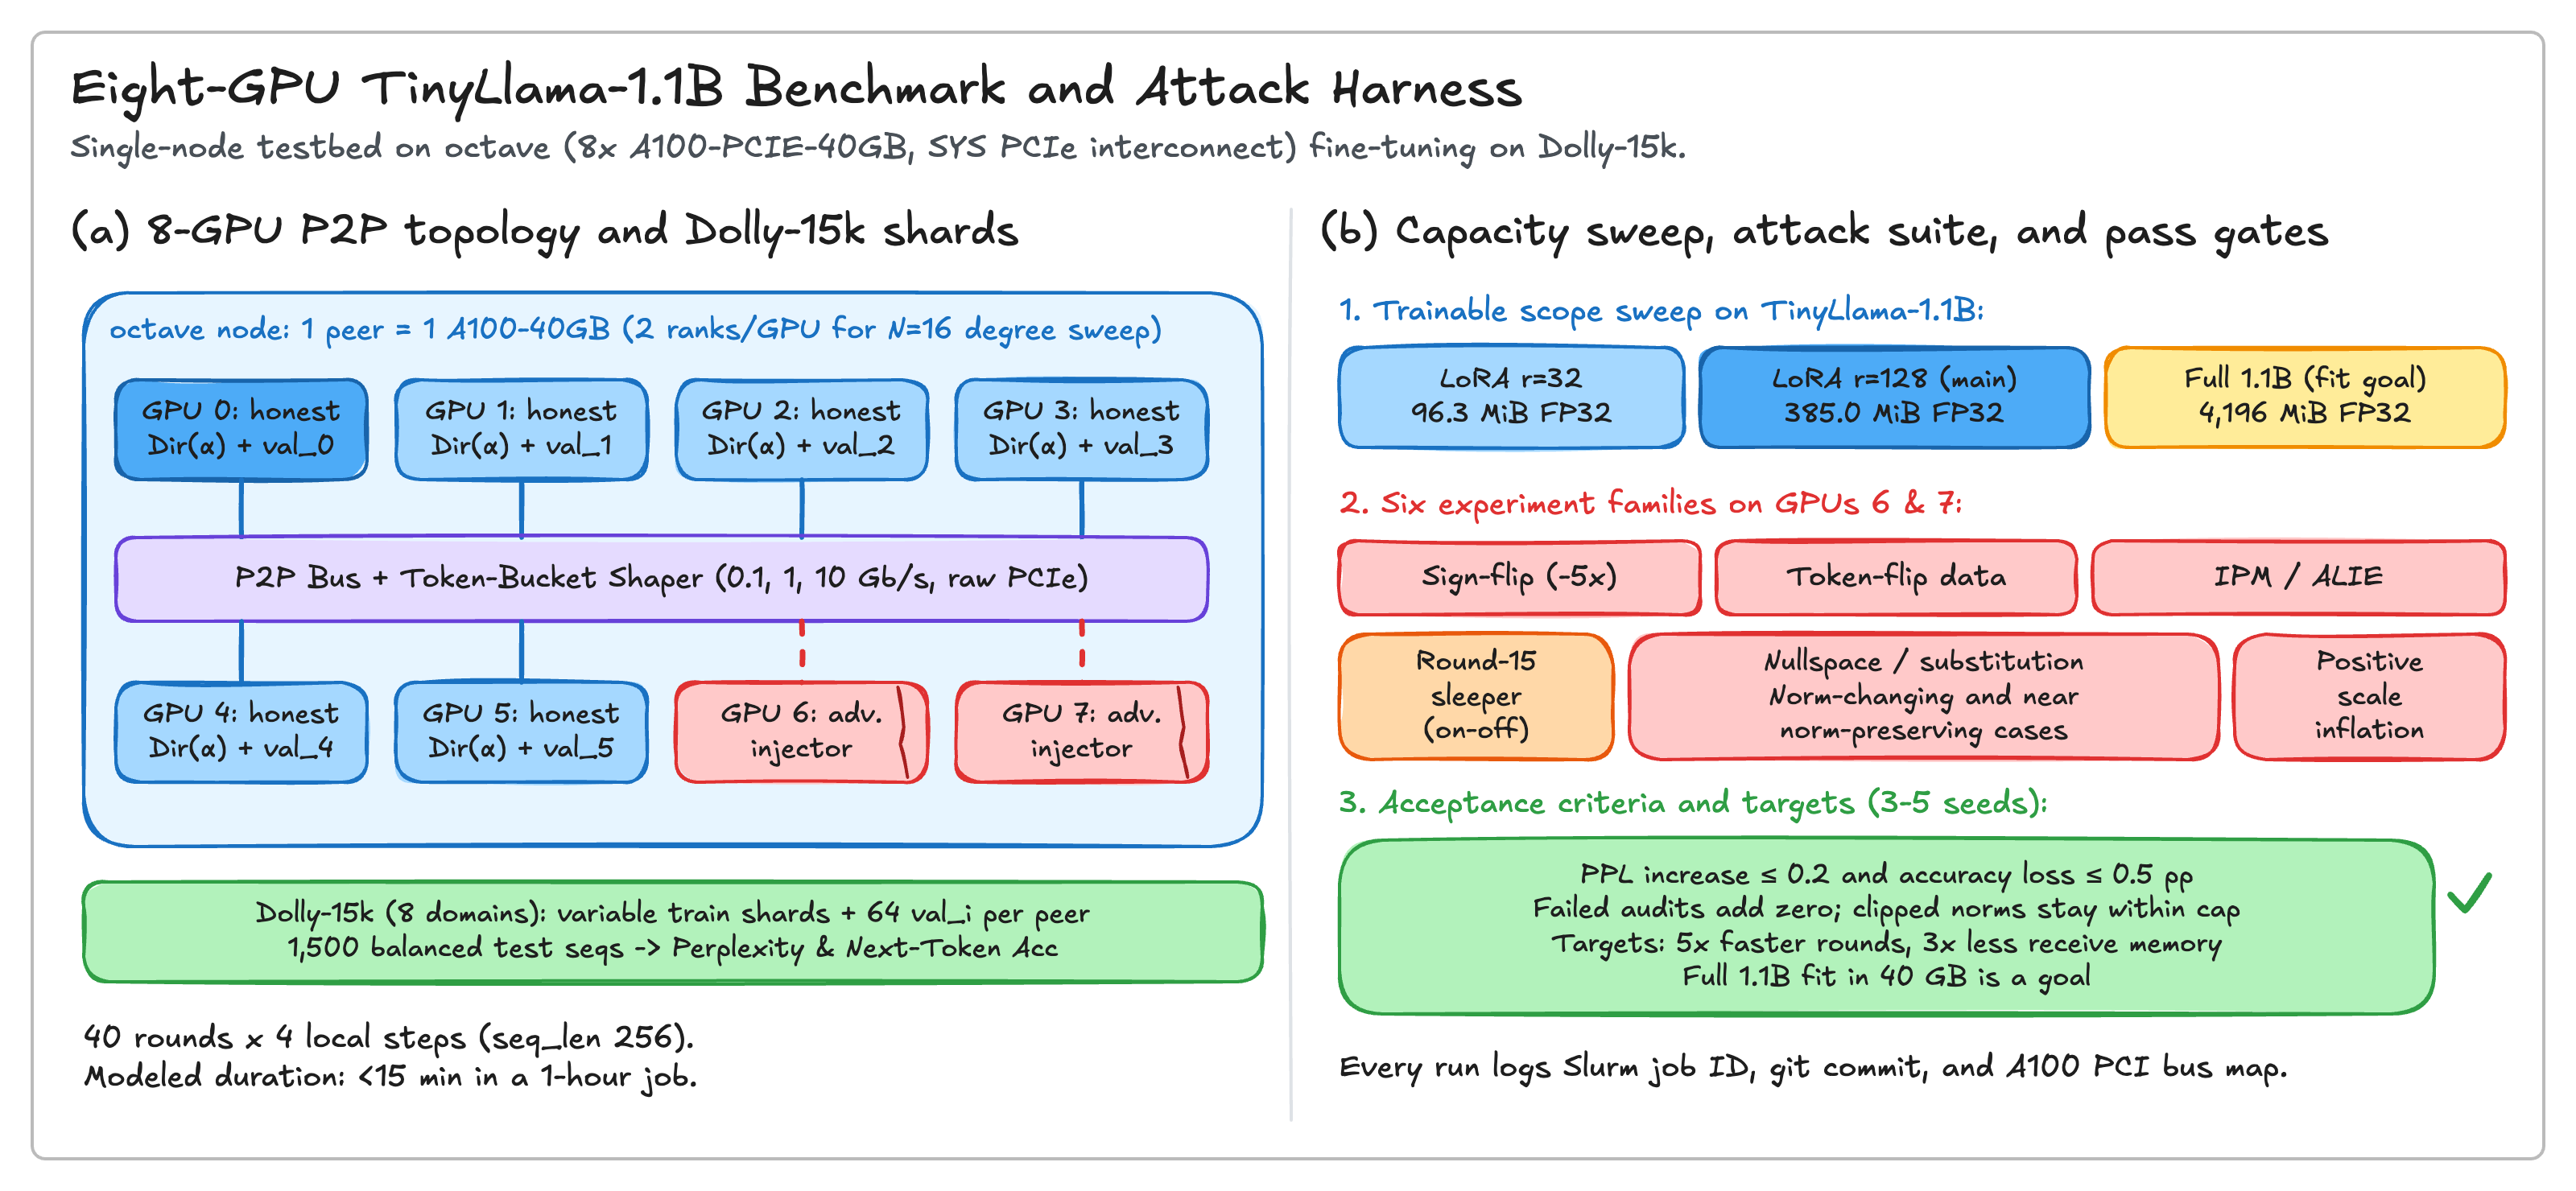
\includegraphics[width=\linewidth]{figures/fig7_eval.png}
  \captionof{figure}{Planned eight-GPU evaluation harness. Honest peers train on Dirichlet-partitioned Dolly-15k shards and reserve local validation sequences. The main configuration uses two Byzantine peers to test six stress families across three trainable scopes.}
  \label{fig:eval}
\end{inlinefigure}

\textbf{Testbed and data.} Figure~\ref{fig:eval} shows the planned testbed: eight NVIDIA A100-PCIE-40GB GPUs on \texttt{octave}, connected via PCIe Gen4 without NVLink. The main configuration places one peer on each GPU in a six-regular graph. A token bucket caps each peer's total receive rate. These caps emulate bandwidth constraints rather than measure an external network.

Dolly-15k contains roughly $15{,}000$ instruction-response examples in eight categories. We will reserve $1{,}500$ category-balanced test examples and partition the rest using a per-category Dirichlet split. The default concentration is $0.1$, with additional splits at $0.05$ and $0.5$ and an IID comparison. Shard sizes vary. We will resample if any peer receives fewer than 80 sequences, the minimum for 64 validation sequences and one training batch, and report the realized shard sizes. Each run uses sequences truncated to 256 tokens and 40 rounds of four AdamW steps at batch size 16. Each peer computes its validation gradient over two batches of 32.

\paragraph{Hypotheses and comparisons.} Within each paired comparison, we will hold the transport, pretrained weights, partition seed, and data order fixed. Batched FP32 TrustGraph-DFL is the primary reference for model quality and receive costs (Table~\ref{tab:baselines}). The sparse baseline tests whether sparsification changes alignment on non-IID shards, while the INT4 baseline isolates the effect of compression. To assess the Pass~1 audit, we will compare the full protocol with a variant that retains screening and clipping but uses sketch-based weights. This comparison tests whether auditing reduces Byzantine acceptance or weight without a substantial increase in honest rejection.

We will ablate the sketch screen, streaming, clipping, and quarantine individually. The dense streaming baseline separates the effect of reduced buffering from that of receiving fewer bytes. The clipping ablation measures the magnitude of accepted updates, while the quarantine ablation measures active neighbor degree and honest connectivity. We will compare timing across receive-rate caps to determine when transferring fewer bytes reduces round time.

\begin{table}[htbp]
  \caption{Planned LLM comparison configurations. TrustGraph variants use the descent-corrected sign convention.}
  \label{tab:baselines}
  \centering\small
  \begin{tabularx}{\linewidth}{@{}P{0.44\linewidth}Y@{}}
    \toprule
    Configuration & Experimental role \\
    \midrule
    Unprotected DFL & Reference without Byzantine filtering. \\
    BALANCE & Distance-based decentralized defense without a validation set. \\
    Batched TrustGraph-DFL (FP32) & Primary uncompressed baseline for quality and receive costs. \\
    Sparse Top-1\% + TrustGraph & Tests whether sparsification weakens alignment on non-IID data. \\
    Blockwise INT4 + TrustGraph & Isolates compression without sketch screening, streaming, or quarantine. \\
    PeerSieve without Pass~1 audit & Uses sketch weights and still clips payloads using their decoded norm. \\
    PeerSieve (complete system) & Evaluates the sketch screen, payload audit, streaming, clipping, and quarantine together. \\
    \bottomrule
  \end{tabularx}
\end{table}

\subsection{Robustness Stress Tests}

The main configuration uses two Byzantine peers. We will sweep from zero to three and report the observed number of Byzantine neighbors per receiver. Let $x_j$ be a clean reference update and $\delta$ a perturbation. Equation~\eqref{eq:attacks} defines the sign-flip and nullspace cases in update space. For encoded payloads, we will measure residual sketch differences rather than assume quantization preserves the nullspace condition.
\begin{equation}
\begin{aligned}
  x_j^{\mathrm{flip}} &= -\gamma x_j, \\
  x_j^{\mathrm{null}} &= x_j+\delta, \qquad \mathcal S_t(\delta)=0 .
\end{aligned}
\label{eq:attacks}
\end{equation}

\begin{enumerate}
  \item \textbf{Sign flip.} Negate an update and amplify it fivefold.
  \item \textbf{Token-flip data poisoning.} Permute target response tokens in the Byzantine peers' training data.
  \item \textbf{Inner-product manipulation.} Test updates near the filter's zero-alignment decision boundary.
  \item \textbf{Sleeper.} Use honest updates for rounds 1--14, then switch to sign flipping in round 15.
  \item \textbf{Nullspace and substitution.} Compare norm-increasing and approximately norm-preserving nullspace cases with payload substitution that changes the canonical sketch. Measure acceptance in each case.
  \item \textbf{Positive scale inflation.} Compare the magnitude of accepted updates with and without clipping under large positive rescaling. Record the realized scale after encoding.
\end{enumerate}

\subsection{Measurements, Projections, and Success Criteria}

\paragraph{Planned measurements.} We will record held-out perplexity and next-token accuracy, rejection rates for honest updates, acceptance rates and aggregate trust weights for Byzantine updates, received bytes, phase times, and peak CUDA memory. Run logs will include the cause of each audit rejection, the size of the largest connected component of honest peers, and the observed active degree. We will time local training, validation, encoding and sketch computation, network wait, and payload audit separately. Convergence runs will use $1$~Gb/s. Separate ten-round timing runs will use $100$~Mb/s, $10$~Gb/s, and unthrottled PCIe. For each configuration and stress case, we will use three to five paired seeds, exclude warm-up from timing, and report the median and range across seeds. We will record the Slurm job ID, Git commit, and GPU PCI bus map for each run.

\paragraph{Analytical memory budget.} Let $D$ be the dense FP32 update size in MiB, $Q$ the compressed size in MiB, and $K$ the neighbor degree. The batched baseline budgets $(K+2)D$~MiB for one dense update per neighbor, the validation vector, and the accumulator. PeerSieve budgets $(2D+Q+4)$~MiB, plus small sketch buffers and state not included in Table~\ref{tab:vram}. The degree sweep will use up to two ranks per GPU to test whether the receive-side tensor buffers remain flat as neighbor degree increases. We will assess full-parameter fit separately at neighbor degree six with one rank per GPU.

\begin{table}[htbp]
  \caption{Predicted receive-side tensor memory in MiB. Training allocations, sketch bookkeeping, and the sender's FP32 error-feedback residual are excluded.}
  \label{tab:vram}
  \centering\small
  \begin{tabularx}{\linewidth}{@{}Yrrrr@{}}
    \toprule
    Trainable scope & FP32 $D$ & Baseline $K=6$ & Baseline $K=12$ & PeerSieve \\
    \midrule
    Rank-32 LoRA & 96.3 & 770.0 & 1,347.5 & 208.9 \\
    Rank-128 LoRA & 385.0 & 3,080.0 & 5,390.0 & 823.6 \\
    Full 1.1B & 4,196.4 & 33,570.8 & 58,748.9 & 8,937.6 \\
    \bottomrule
  \end{tabularx}
\end{table}

For full-parameter tuning, the projected receive-side tensor buffers occupy 8.73~GiB and the separate FP32 residual occupies 4.10~GiB. An assumed remaining training footprint of 18~GiB yields about 30.8~GiB before other overheads. This budget does not establish that the run fits. We will measure the end-to-end peak, including training allocations and allocator effects.

\paragraph{Success criteria.} We will assess the complete system against the following targets:
\begin{enumerate}
  \item \textbf{Accuracy.} In each tested stress case, final held-out perplexity is no more than $0.2$ above the FP32 baseline and next-token accuracy is no more than $0.5$ percentage points below it.
  \item \textbf{Robustness.} Failed payload audits never modify the aggregate, and accepted payloads respect the norm cap. Honest rejection exceeds the baseline by at most five percentage points. We will report accepted Byzantine payloads, their aggregate weight, and the corresponding test metrics.
  \item \textbf{Efficiency.} At neighbor degree six with rank-128 LoRA and $1$~Gb/s, median round time is at most one fifth of the batched FP32 baseline's, and measured receive-side tensor memory is at most one third of the baseline's.
  \item \textbf{Scale.} Full-parameter tuning at neighbor degree six completes on one 40~GB A100 per peer without running out of memory.
\end{enumerate}

In the scenario in Table~\ref{tab:round}, the baseline is projected to take 9.6 times as long per round and use 3.7 times as much receive-side tensor memory as PeerSieve. The realized gains depend on local training time, how many payloads pass screening, and the cost of deterministic reductions and two-pass decoding.

\section{Conclusion}

PeerSieve screens updates before transfer without relying on a sketch alone for aggregation. Its design replaces per-neighbor dense buffers with a reusable staging buffer and tile at the cost of a second local decoding pass. The proposed evaluation will test whether the communication and memory savings outweigh the audit overhead and whether the filters preserve model quality under heterogeneous data and Byzantine behavior.

\clearpage
\bibliographystyle{unsrtnat}
\bibliography{references}
\end{document}
